\subsection{Daten und Analyse}
	Die in den Abbildungen \ref{fig:Kreiselunten}, \ref{fig:Kreiselmitte} und \ref{fig:Kreiseloben} eingezeichneten Steigungen der linearen Anpassungen sind in \ref{tab:Kreisel} zusammengefasst.
Man erkennt in den Abbildungen das einige Werte sehr stark von der Anpassung abweichen, dies lässt einen Fehler in der Durchführung vermuten.
\begin{table}[h]
		\caption{Messwerte für die verschiedenen Positionen des Zusatzgewichtes}
		%{Zu sehen sind die Werte für die Steigung die Kraft für die drei unterschiedlichen Positionen sowie die Masse der Kugel, Radius der Kugel sowie die Länge l.}
	\scriptsize 
	\begin{tabular}{|c|c|c|c|c|c|}
		\hline
		Position & $\Delta T_p/\Delta \omega$ & Kraft $F$ & Radius $R$ & Masse $m$ &Länge $l$\\
		\hline
		Unten (1) & \SI{5,13+-0.09e-2}{1/s^2} & \SI{0,144+-0,005}{N} & \SI{25,39+-0,01}{mm} & \SI{512,240+-0,003}{g}& \SI{84.82+-0,02}{mm}\\
		\hline
		Mitte (2)& \SI{4,31+-0,02e-2}{1/s^2}& \SI{0,166+-0,005}{N} & \SI{25,39+-0,01}{mm} & \SI{512,240+-0,003}{g}&\SI{84.82+-0,02}{mm}\\
		\hline
		Oben (3) & \SI{3,59+-0,03e-2}{1/s^2}& \SI{0,220+-0,005}{N} & \SI{25,39+-0,01}{mm} & \SI{512,240+-0,003}{g}&\SI{84.82+-0,02}{mm}\\
		\hline
		\end{tabular}
	\label{tab:Kreisel}
\end{table}
\normalsize
\begin{figure}[h]
	\centering
	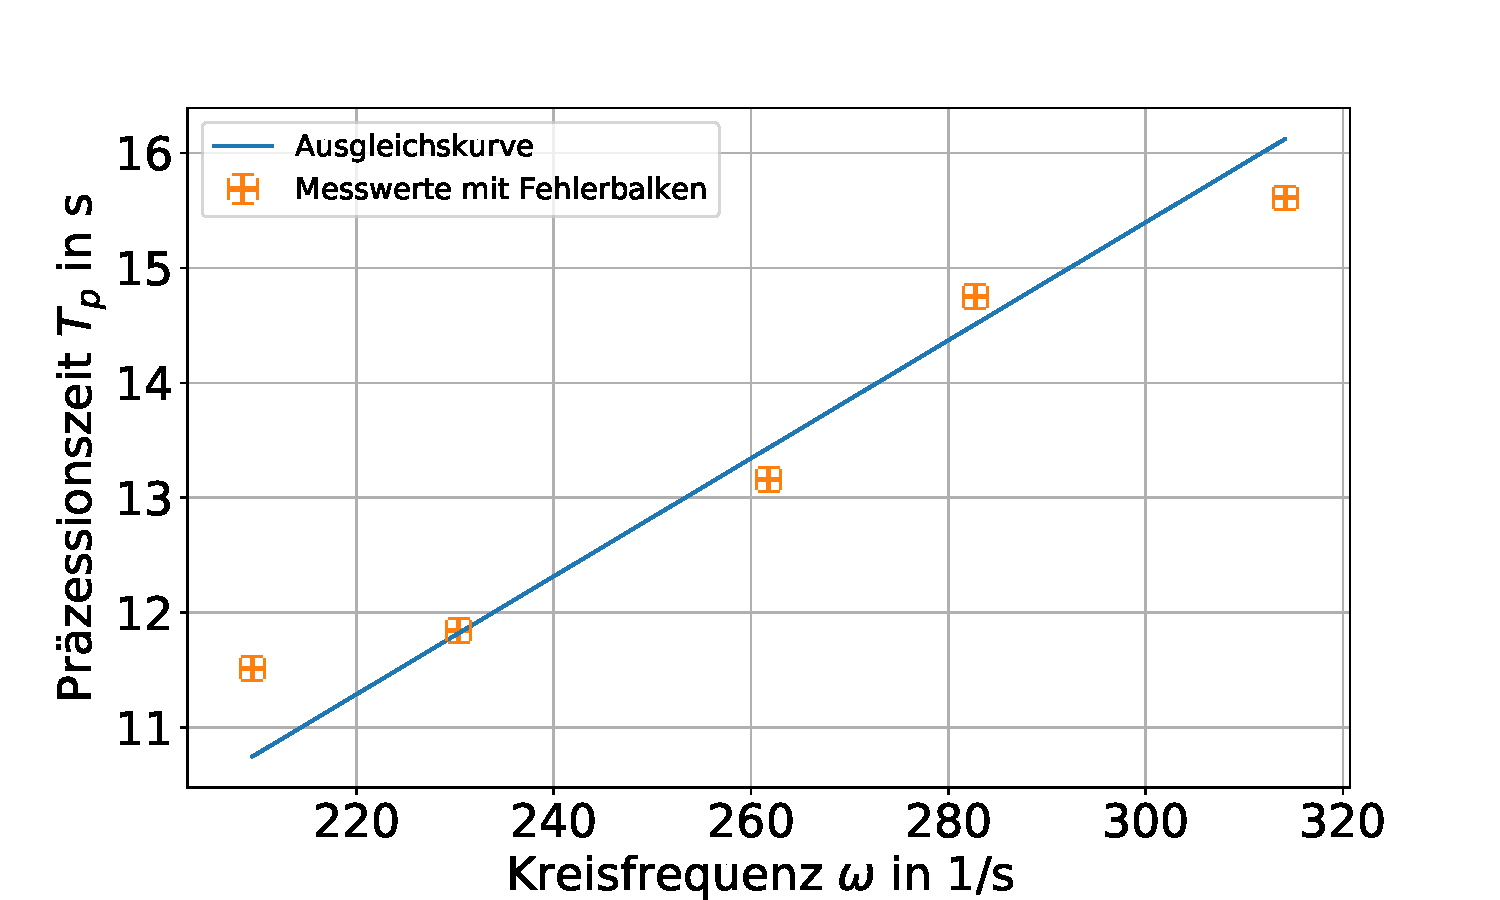
\includegraphics[width=0.9\textwidth]{res/sproHzunten.pdf}
	\caption{Aufgetragen ist die die Präzessionzeit $T_p$ gegen die Kreisfrequenz $\omega$ bei Positionierung des Zusatzgewichtes bei Position 1.}
	\label{fig:Kreiselunten}
\end{figure}
\begin{figure}[h]
	\centering
	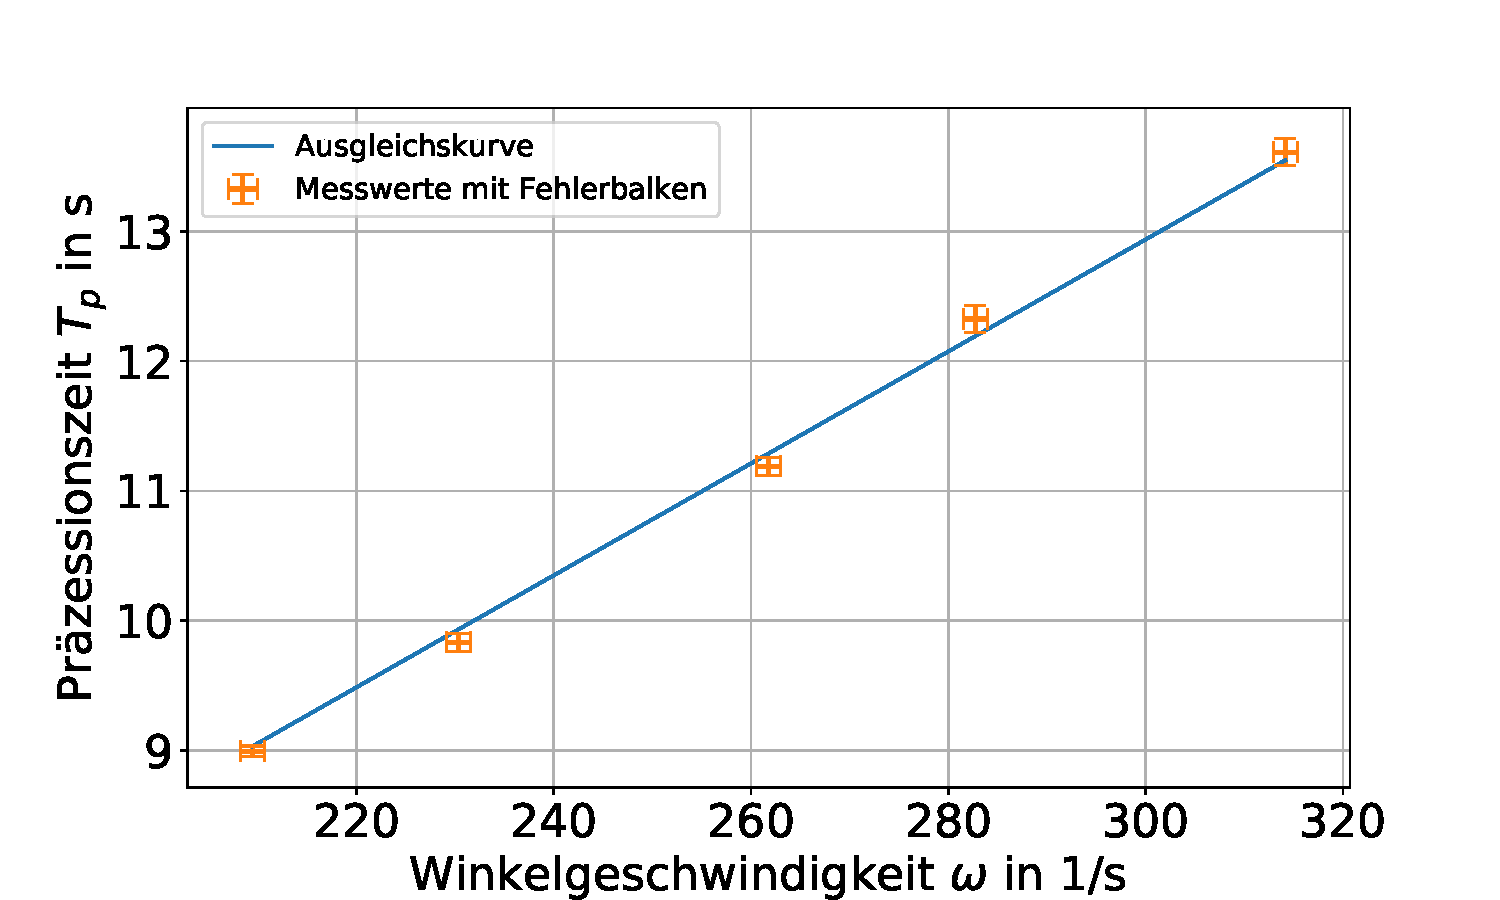
\includegraphics[width=0.9\textwidth]{res/sproHzmitte.pdf}
	\caption{Aufgetragen ist die die Präzessionzeit $T_p$ gegen die Kreisfrequenz $\omega$ bei Positionierung des Zusatzgewichtes bei Position 2.}
	\label{fig:Kreiselmitte}
\end{figure}

\begin{figure}[h]
	\centering
	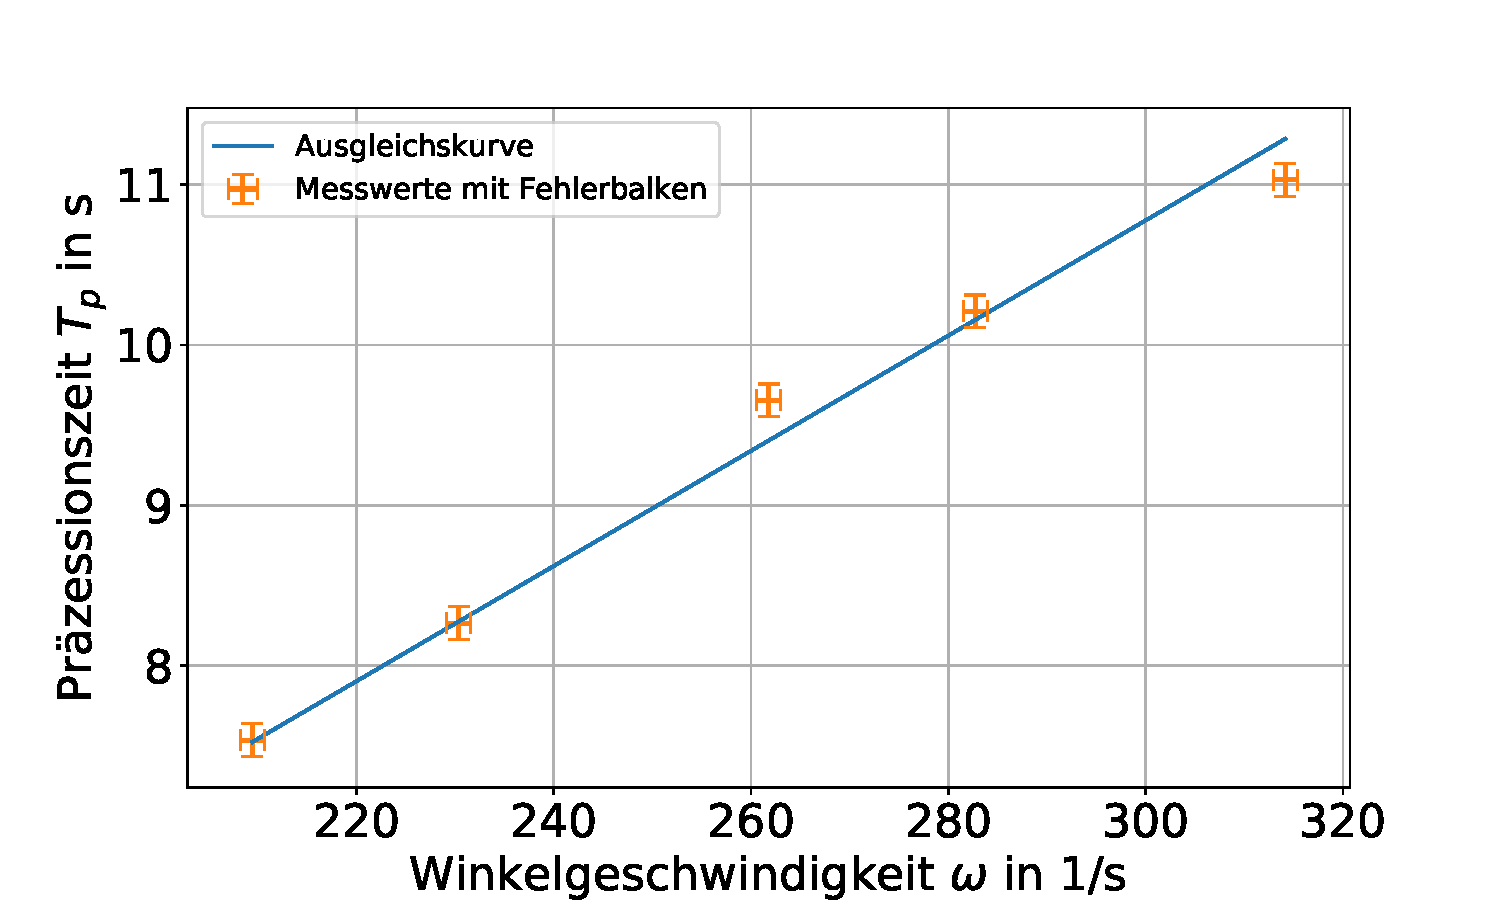
\includegraphics[width=0.9\textwidth]{res/sproHzoben.pdf}
	\caption{Aufgetragen ist die die Präzessionzeit $T_p$ gegen die Kreisfrequenz $\omega$ bei Positionierung des Zusatzgewichtes bei Position 3.}
		\label{fig:Kreiseloben}
	\end{figure}
Im nächsten Schritt wurde das Produkt der Länge $l$ und der Kräfte $F$ gegen den Kehrwert der Steigungen aus den Abbildungen  \ref{fig:Kreiselunten}, \ref{fig:Kreiselmitte} und \ref{fig:Kreiseloben} aufgetragen. 
Daraus resultierte die Abbildung \ref{fig:Kreisel}.
Man erkennt das die lineare Anpassung die drei Messwerte nicht gut approximiert, da nur einer von drei Punkten im Rahmen der Standartunsicherheit auf der Ausgleichsgeraden liegt. Dies ist, wie schon vorher erwähnt, auf einen bei der Durchführung vermuteten Fehler zurückzuführen.
%Über den in Kapitel \ref{kap:KreiselMethoden} bereits genannten Zusammenhang zwischen der Steigung aus der Abbildung und dem Trägheitsmoment. Dieser Zusammenhang lautet: $\frac{a}{1\pi}=J$ wobei es sich bei a um die Steigung handelt. Somit erhält man für $J_{exp.}$ den folgenden Wert: $J_{exp.}=\SI{1,0194+-0,0319e-4}{kg \cdot m^2}$. 
Durch den in \ref{eq:zusJlF} beschriebenen Zusammenhang zwischen der Steigung der Geraden in \cref{fig:Kreisel} und dem Trägheitsmoment erhält man:  $J_{exp.}=\SI{1,0194+-0,0319e-4}{kg \cdot m^2}$. 
Dieser Wert wurde dann mit dem $J_{theo.}$ verglichen, der mithilfe der folgender Gleichungen berechnet wurde:
\begin{align}
	J_{Kugel}=\frac{2}{5}mr^2\\
	J_{exp}=J_{Kugel}+J_{Zusatz}
	\label{eq:J}
\end{align}
Masse und Radius der Kugel wurden wie in Kapitel \ref{kap:KreiselMethoden} beschrieben gemessen und das Trägheitsmoment der Stange und des Zusatzgewichtes war mit $J_{Zusatz}=\SI{15}{g \cdot cm^2}$ angeben. Somit ergab sich dann folgender Wert: $J_{theo.}=\SI{1,3356+-0,0004e-4}{kg \cdot m^2}$. Wie man erkennt unterscheiden die beiden Werte für das Trägheitsmoment um ca. 30 \%.
\begin{figure}[h]
	\centering
	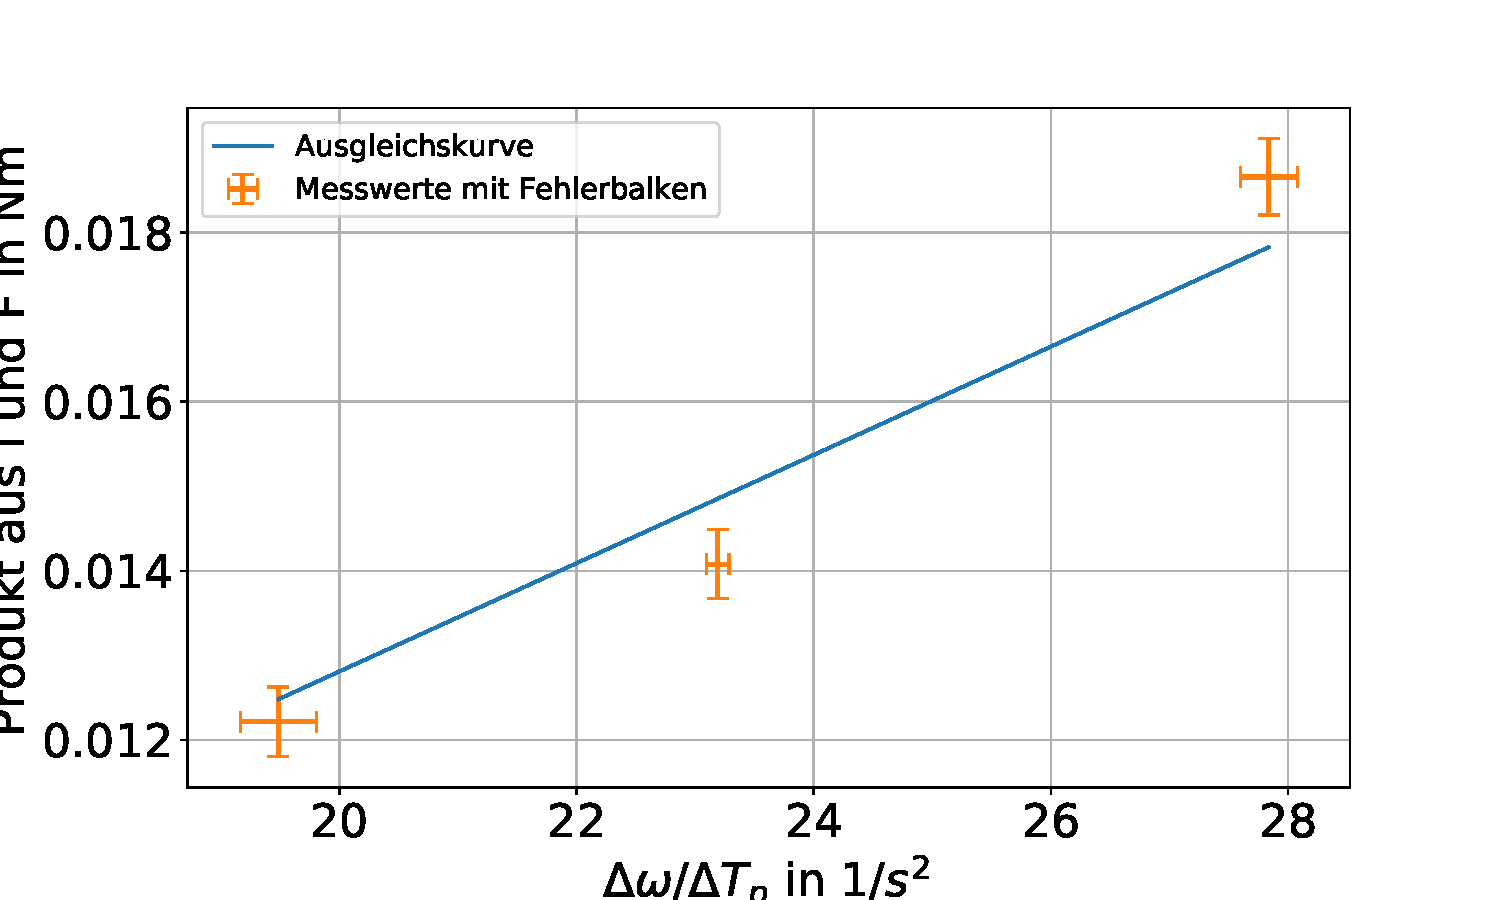
\includegraphics[width=0.9\textwidth]{res/wtgegenlF.pdf}
	\caption{Aufgetragen ist das Produkt l mal F gegen $\frac{\Delta \omega}{\Delta T_p }$.} 
	\label{fig:Kreisel}
\end{figure}
